\documentclass{article}
\usepackage[utf8]{inputenc}

\title{Quadratic Functions}
%\author{Your Name}
%\date{November 2016}

\usepackage{natbib}
\usepackage{graphicx}

\begin{document}

\maketitle

\section{Quadratic Functions}
When $a \ne 0$, quadratic quation $ax^2 + bx + c = 0$ has two solutions and the roots are
$x = {-b \pm \sqrt{b^2-4ac} \over 2a}.$ 

$ \begin{array}{rcl}
y & = & a x^{2}+bx+c\\
  & = & a\left(x^{2}+2\times\frac{b}{2a}x+\frac{c}{a}\right)\\
  & = & a\left(x+\frac{b}{2a}\right)^2 - \frac{b^2}{4a} + c
\end{array} $ 

Vertex of the parabola, $y = f(x)$ is $\left(-\frac{b}{2a}, c - \frac{b^2}{4a}\right)$.

\begin{center}
\begin{tabular}{|l|l|}
\hline
 $d = b^2 - 4ac$ & comment about roots \\ 
 \hline
 $d>0$ & roots are real and distinct \\  
 \hline
 $d = 0$ & roots are real and same \\
 \hline
 $d<0$ & roots are complex \\
\hline
\end{tabular}
\end{center}

\begin{figure}[h!]
\centering
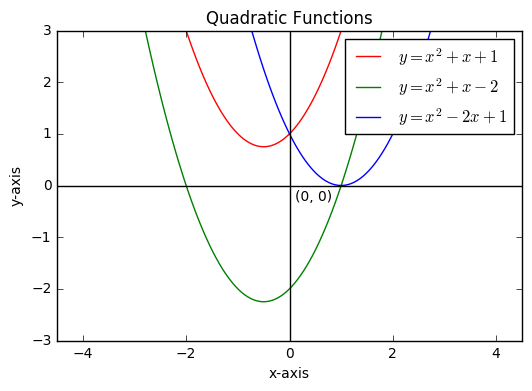
\includegraphics[scale=.4]{quadraticplots.png}
\caption{Quadretic Functions}
\label{fig:quadretic}
\end{figure}

\section{Conclusion}
Congratulations!!! You are now a \LaTeX~ user.

\end{document}

